\graphicspath{{chapters/analysis/images/}}
\label{sec:fitting_data}
\section{Fitting Data}
Icecube analyses are developed blindly in order to minimize bias.
This proceeds in a few distinct stages, each described separately here.

\unsure{may just remove the burn sample crap. its so out of date that its too weird to go back and redo it.}
\label{subsec:burn_sample}
\subsection{Burn Sample Fits: Testing the Fitting Code}
Analyzers are initially restricted to a small fraction of the full dataset while developing the event selection and fitting codes.
The size of the burn sample, here limited to 1\% of the total dataset, is selected in order to provide reasonable statistics while maintaining limited sensitivity to the final physics parameters.
Once end-to-end tests are completed using solely simulated events, this small sample, known as the \emph{burn sample}, is fit in order to verify that results obtained are reasonable.

\improvement{blahdy blahdy blahdy. no point spending time here if i may just kill it}


\label{subsec:blind_fits}
\subsection{Blind Fits: Checking the Goodness-of-Fit}
Once the burn sample tests are complete, the next stage is to perform what is known as a \emph{blind fit}.
The concept, developed for oscillation analyses in IceCube, exists as an intermediate stage between the low-sensitivity burn sample tests and the final fit 
Unlike the burn sample fits, the blind fits use the full data sample for testing.
All systematics are included in the fit as normal.
The final physics parameters, in this case the oscillation parameters and the $\nu_\tau$ normalization, are allowed to fit freely, but the final results are obfuscated.
The goodness-of-fit and systematics values are free for investigation.
Analyzers are free to move onto a request for full unblinding if the goodness-of-fit exceeds 5\%.
If the goodness-of-fit is significantly lower than this limit, the sample and fit is investigated further to identify any potential issues or oversights.
The blind fit is a test designed to look for problems prior to full unblinding in order to implement necessary fixes while remaining blind to the effect on the final result.

The goodness-of-fit, known more informally as the p-value associated with the fit, may be calculated via two closely-related methods.
An ensemble of Monte Carlo trials is fit and the resulting $\chi_{FS}^2$ values are used.
The fraction of trials with $\chi_{FS}^2$ larger than that observed in data gives the first p-value.
The second method uses SciPy \findref{scipy} to fit a $\chi^2$ distribution. 
The p-value may then be calculated from the continuous distribution by finding the total probability of observing a fit with a $\chi_{FS}^2$ value equally or worse than the data fit, ${P_2\left(\chi_{FS}^2 \geq \left(\chi_{FS}^2\right)_{Data}\right)}$.

The first method generally will yield more accurate results, particularly if the resulting distribution is poorly fit by a simple $\chi^2$ distribution. 
If the fit is particularly poor, a large number of trials may be necessary in order to calculate an accurate p-value.
In these cases, the second method may be used to provide an estimate of the p-value of the fit.

During the first work with blind fits, this analysis used a wide range of reconstructed energies, including events up to 800 GeV in order to better constrain systematics terms in the non-oscillating higher energy regions.
Blind fits in the GRECO analysis initially showed significant disagreement between the data and simulation, with a goodness-of-fit of ${10^{-7}}$.
Investigations yielded new discoveries about both the calibration of the Monte Carlo simulation and previously-unknown erroneous events in the data.


\label{section:tau_results}
\section{Results from the Search for Appearance}
After the removal of the flaring DOM events, the correction of bedrock events, and the elimination of the charge in the PegLeg fit, a new blind fit was performed and the goodness-of-fit was again tested.
The resulting $\chi^2_{FS}$ for the charged-current only and neutral-current + charged-current fits were 127.095 and 127.623 respectively.
One thousand trials were run for each fit using the updated sample, yielding estimates of the probability density function shown in \needfig{PDFs for gof}.
The data is well-described by the systematics set, with a pvalue of approximately 57\% for both fits.
The full map of the ${\chi^2_{FS}}$ values is shown in Figure~\ref{fig:chi2_map}.
No single region of disagreement is visible, indicating that there are no significant remaining unmodeled systematic uncertainties.

With the observation of good fit p-values, the final results for both the CC-only and NC+CC fits were fully unblinded.
Both results, shown in Figure~\ref{fig:final_contour_cc} and Figure~\ref{fig:final_contour_nccc}, fit lower than expected from unitary 3-flavor oscillations, although both are consistent with such a model.

The final value of the systematics, shown numerically in Table~\ref{tab:bestfit_systematics} and graphically in Figure~\ref{fig:syst_pulls}, are within 1${\sigma}$ of the expectation at the best-fit points.
Many systematics were expected to be determined primarily from the data instead of from priors. 
Figures~\ref{fig:posteriors_cc} and \ref{fig:posteriors_nc_cc} shows the expected values of each systematic for 1000 trials.
The shaded band shows the assumed 1${\sigma}$ prior range for each of the parameters, if present.
Not only are all systematics within the relevent priors, but most systematics fit within the expected posteriors.

\begin{figure}{}
	\centering 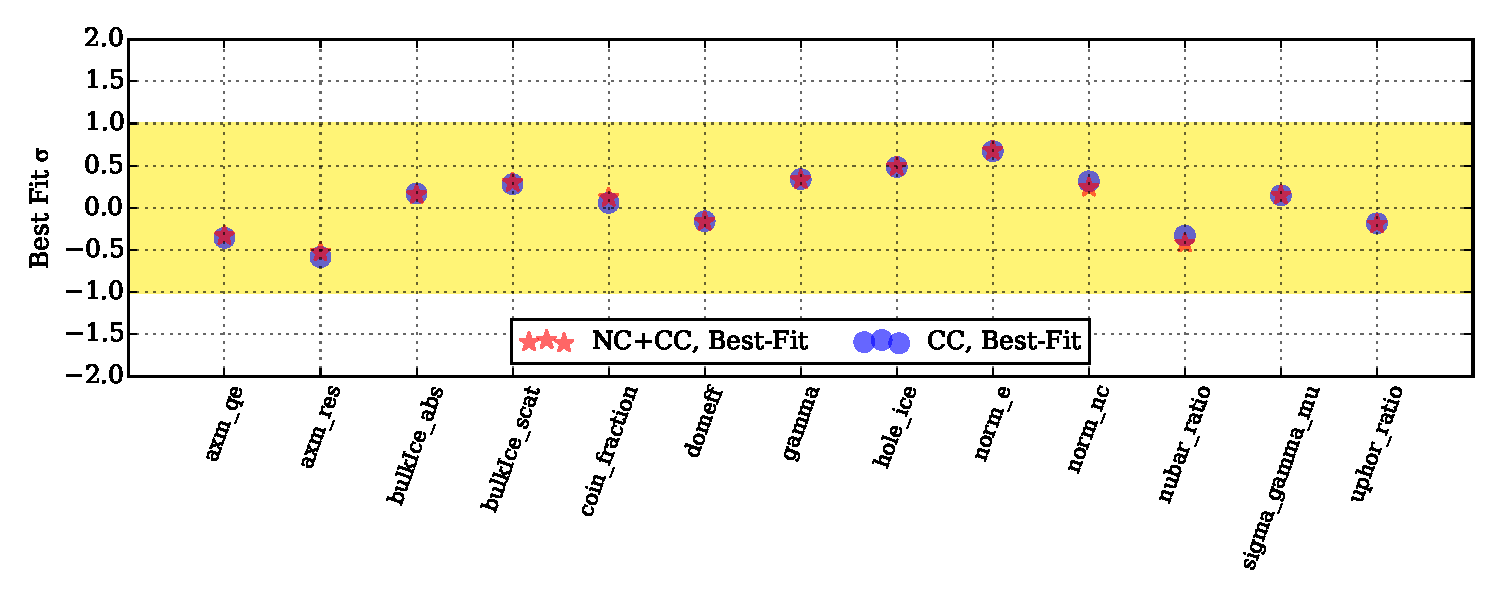
\includegraphics[width=\textwidth]{pulls.pdf}
	\caption{The value of each systematic with priors. The best-fit values are shown for each while the priors are shown by the yellow band. The CC and NC+CC fits are highly correlated, as expected, with very little difference in the systematics best-fit values. All values fit well within the expected 1$\sigma$ ranges.}
	\label{fig:syst_pulls}
\end{figure}

\begin{figure}{}
	\centering 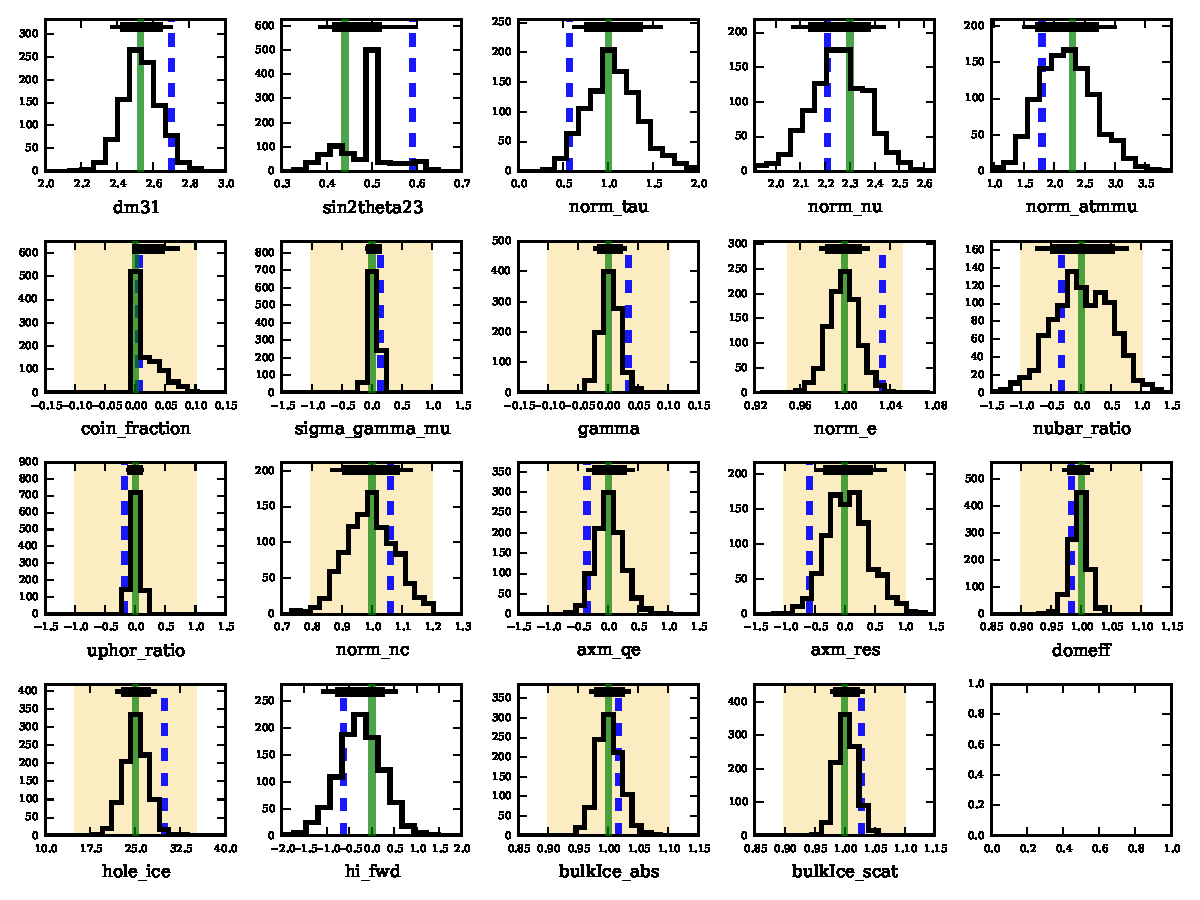
\includegraphics[width=\textwidth]{cc_systematics.pdf}
	\caption{A comparison of the posterior expected from trials to the final data fit value for each parameter for the CC-only fit. The trials used to build the posterior distribution in each parameter assume baseline values for systematics, $N_\tau^{CC}=1$, and Nu-Fit 2.2 values \cite{NuFit_2.2}. The green vertical line shows the true injected value. The blue dotted line shows the best-fit value from data. The black bar shows the 1$\sigma$ and 90\% ranges calculated from the posterior distribution.}
	\label{fig:posteriors_cc}
\end{figure}

\begin{figure}{}
	\centering 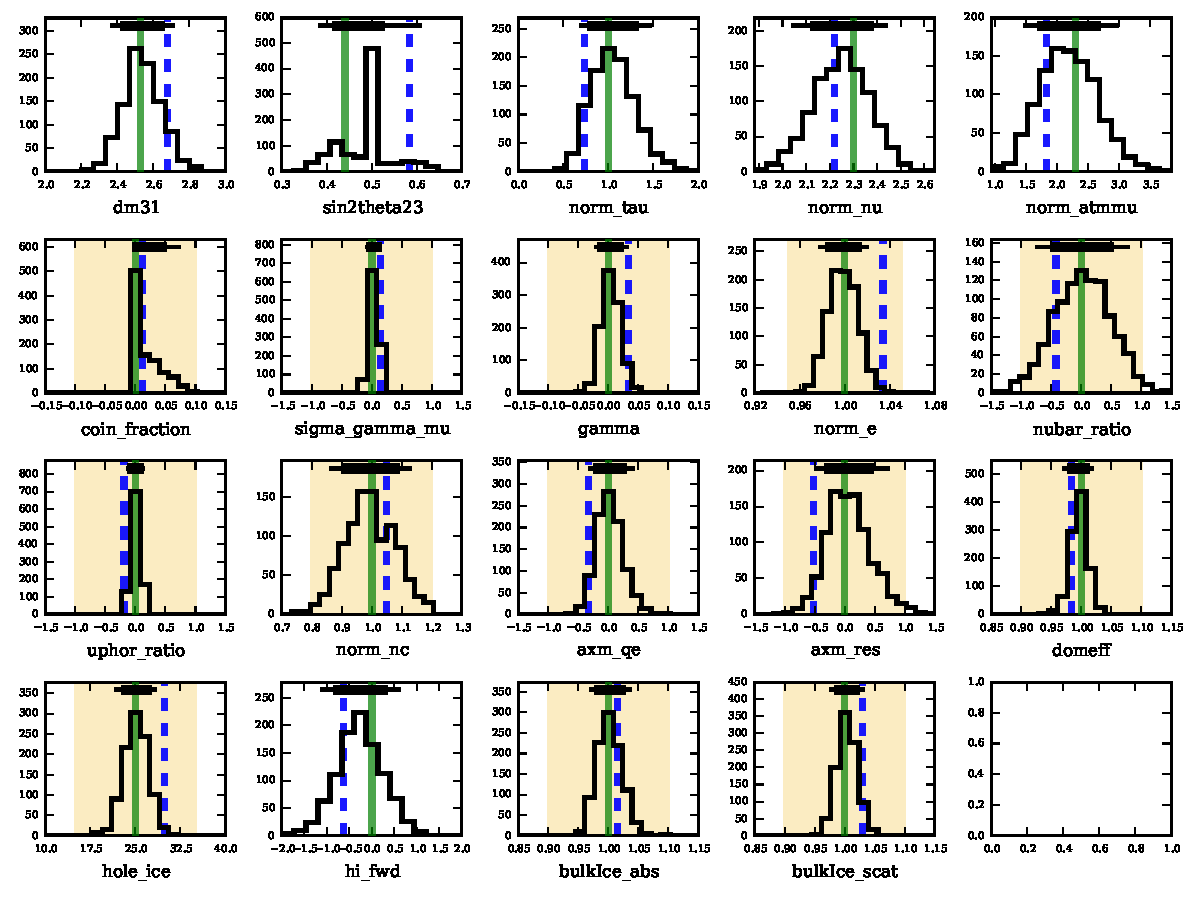
\includegraphics[width=\textwidth]{nc+cc_systematics.pdf}
	\caption{A comparison of the posterior expected from trials to the final data fit value for each parameter for the NC+CC fit. The trials used to build the posterior distribution in each parameter assume baseline values for systematics, $N_\tau^{NC+CC}=1$, and Nu-Fit 2.2 values \cite{NuFit_2.2}}
	\label{fig:posteriors_nc_cc}
\end{figure}

\begin{landscape}
\begin{table}[]
\centering
\resizebox{\textwidth}{!}{%
\begin{tabular}{@{}lllllll@{}}
\toprule
\multirow{2}{*}{Parameter Type} & \multirow{2}{*}{Fit Parameter}    & \multirow{2}{*}{Units} & \multirow{2}{*}{Prior} & \multicolumn{1}{c}{\multirow{2}{*}{Disappearance}} & \multicolumn{2}{l}{Appearance} \\
                                &                                   &                &             & \multicolumn{1}{c}{} & CC-Only        & NC+CC         \\ \midrule
Oscillations               & $\Delta m^2_{32}$     & $10^{-3}$ $eV^2$ & -        & 2.548           & 2.625          & 2.602         \\
                                & $\sin^2 \left(\theta_{23}\right)$  & -          & -        & 0.576           & 0.590          & 0.584         \\ 
                                & $N_\tau$                   & -               & -                      & 1.0 (Fixed)    & 0.566          & 0.733         \\\midrule
Cross-section            & Axial Mass (QE)           & $\sigma$  & 0 $\pm$ 1.0    & -0.250          & -0.357         & -0.332        \\
                                & Axial Mass (RES)         & $\sigma$   & 0 $\pm$ 1.0   & -0.3737        & -0.583         & -0.526        \\
                                & $N_{NC}$                  & -                & 1 $\pm$ 0.2   & 1.016           & 1.063          & 1.048         \\ \midrule
Neutrino Flux             & $\nu_\mu$ Norm       & Years         & -                     & 2.151           & 2.210          & 2.219         \\
                                & $\nu_e$/$\nu_\mu$  & -               & 1 $\pm$ 0.05  & 1.031           & 1.034          & 1.033         \\
                                & $\gamma_\nu$          & -               & 0 $\pm$ 0.10  & 0.045           & 0.034          & 0.033         \\
                                & $\nu$/$\bar{\nu}$    & $\sigma$  & 0 $\pm$ 1.0     & -0.700         & -0.330         & -0.422        \\
                                & Up/Hor                       & $\sigma$  & 0 $\pm$ 1.0    & -0.207          & -0.184         & -0.191        \\
                                & $f_{Coincident}$        & \%            & 0 + 0.1            & 0.027           & 0.006          & 0.012         \\ \midrule
Muon Flux                  & $\mu$ Norm              & Years        & -                      & 1.845           & 1.795          & 1.830         \\
                                & $\gamma_{CR}$       & $\sigma$  & 0 $\pm$ 1.0    & 0.113          & 0.148          & 0.148         \\ \midrule
Detector                   & DOM Efficiency            & -               & 1.0 $\pm$ 0.1 & 0.980          & 0.984          & 0.984         \\
                                & Hole Ice (Flasher)        & -               & 25 $\pm$ 10   & 30.526        & 29.833         & 29.894        \\
                                & Forward Scattering      & -               & -                      & -0.839         & -0.638         & -0.630        \\
                                & Absorption                  & \%           & 1.0 $\pm$ 0.1  & 1.014          & 1.017          & 1.016         \\
                                & Scattering                   & \%           & 1.0 $\pm$ 0.1   & 1.033         & 1.028          & 1.030         \\ \bottomrule
\end{tabular}%
}
\caption{The best-fit systematics values for each nuisance parameter in the fit. The corresponding parameters for $N_\tau=1$ (ie, the disappearance fit) are included for reference. The CC-only and NC+CC fits are highly correlated, as expected. }
\label{tab:bestfit_systematics}
\end{table}
\end{landscape}





\label{section:other_measurements}
\section{Complementary Measurements from This Analysis}

\label{subsec:oscil_results}
\subsection{Oscillation Parameters}
Thanks to significant contributions from others \findref{future reference to martin, elim's theses}, dedicated measurements of the atmospheric mixing parameters have also been performed using the GRECO selection.
In these measurements, the value of ${N_{\nu_\tau}}$ remains fixed to unity.
The derived results are therefore directly comparable to results from other oscillation experiments.

\label{subsubsec:disappearance_results}
\subsubsection{$\nu_\mu$ Disappearance Results}
Using similar tools as the appearance analysis, a complementary search for ${\nu_\mu}$ disappearance was performed \findref{elim's thesis}.
The measurement of the disappearance parameters, ${\Delta m^2_{3j}}$ and ${\theta_{23}}$, used an identical choice of binning and systematics set as the appearance search described above.
The $\chi^2_{FS}$ statistic was found by minimization with the iMinuit package \findref{iminuit} across a grid of values arranged linearly in ${\Delta m^2_{3j}}$ and ${sin^2\theta_{23}}$ covering both octants.
At each point, the disappearance parameters were fixed during minimization.
Both the normal and inverted ordering are tested separately.

The result is shown in \needfig{elim's result!} with comparisons to previous atmospheric oscillation measurements by IceCube \findref{icecube 2017 result}, Super-Kamiokande \findref{superk 2015 oscillation result} and the MINOS experiment \findref{minos oscillation with atm}.
Results from accelerator measurements are shown from the ${NO\nu A}$ \findref{nova oscillation} and T2K \findref{t2k oscillation result} experiments.
All results show the 90\% contour around the best-fit point.
The GRECO result mildly prefers the normal ordering and the second octant, although maximal mixing (${sin^2\theta_{23}=0.5}$ is well within the best-fit contours.

The GRECO result improves upon the most recent IceCube result significantly, particularly in the measurement of the mass splitting.
Both results are statistically consistent with one another, although the GRECO result perfers a larger mass splitting than the previous result.
Global fits, which prefer a value of the mass splitting of ${2.494^{+0.033}_{-0.031}}$ as of the time of this writing \findref{nufit 3.2}, favor the new GRECO result over the previous IceCube result.

Precise measurements of the atmospheric mixing angle continue to elude us, however.
While the GRECO result provides competive constraints on the mixing angle, no significant improvement is observed.

\label{subsubsec:nmo_results}
\subsubsection{Mass Ordering}
In order to quantify the preference for the mass ordering, a dedicated measurement using the GRECO sample was performed \findref{martin's thesis}.
This measurement included numerous differences relative to the appearance and disappearance measurements.
Only upgoing reconstructed GRECO events were included, although the energy range was extended to 3-100 GeV.
All simulation templates were smoothed during the analysis using a dedicated implementation of the kernal density estimation technique implemented in the C++ programming language \findref{martin's kdes from the aachen group. who did that?}.
This code, unlike the SciPy KDE implementation used in \ref{sec:kde_filtering}, includes functionality for weighted event samples and variable bandwidth estimation.

The systematics set used in the mass ordering analysis was identical to that of the disappearance measurement, with the value of ${N_{\nu_\tau}}$ fixed to unity.
Systematics included in the mass ordering measurement were applied using a parallel branch of the OscFit code used in the appearance measurement.

Statistical uncertainties arising from the simulation statistics were estimated using a bootstrapping technique included in the KDE implementation.
The test statistic used in the mass ordering measurement was defined to be the numerical convolution between the Poissonian uncertainty due to the expected event count and a Gaussian model of the bootstrapped Monte Carlo statistical uncertainty.

Unlike the appearance and disappearance measurements, the neutrino mass ordering is not a continuous parameter. 
The calculation of a final significance proceeds following the method described in \findref{pingu paper and/or pisa paper describing nmo measurement}, a full description of which is beyond the scope of this work.
Using GRECO events, a good fit is obtained at the best-fit point with a pvalue of approximately 80\%.
Using the cited technique, a weak preference for the normal mass ordering is found at approximately 0.3${\sigma}$ \unsure{Need martin's final result!}

\label{subsec:syst_constraints}
\section{New Constraints on Detector Systematics}
The statistics available in the GRECO dataset provide a unique chance to derive new constraints on systematic variables.
For each of the parametrized detector systematics, a scan was performed to evaluate constraints from the dataset.
In all cases, the value of ${N_{\nu_\tau}}$ remained fixed to unity.
The results of these scans are shown in \needfig{chi2 scans of the detector systematics to show greco constraints on domeff, holeice, hifwd, absorption, and scattering}.

These new constraints imply new, tighter limits derived from fits to the detector data.
They do have limitations, however.
During the parametrization process, all systematics were assumed to be uncorrelated, which is unlikely to be the case in practice.
The DOM efficiency and absorption properties in the ice are known to have correlations in dedicated calibration work in the detector, for example.
These correlations are included in the prior uncertainties for each parameter.
Although

Each also assumes an accurate modeling of the effects in question.
All effects are assumed to equally apply to the entire detector.
Bulk changes of the properties associated with each systematic are assumed to be more important than the spread of uncertainties for each DOM (DOM efficiency, hole ice parameters) or layer in the ice (absorption, scattering).
This assumption indicates limited insight may be gained.
Testing the properties for each DOM is unlikely to be within the statistical reach of any dataset in the foreseeable future given the number of DOMs in the detector.

The new constraints from GRECO demonstrate significant power in the dataset to identify new effects like those discussed in \ref{subsec:blind_fits}.
The dataset provides the collaboration with a novel set of low energy events sensitive to evaluate detector properties.
These new constraints may be used in future analyses to limit systematic uncertainties affecting other measurements.

\label{subsec:implications}
\subsection{Implications and Future Work}
There exist various ways to interpret the value of ${N_{\nu_\tau}}$. 
The value of the tau neutrino normalizations in the exclusive and inclusive channels \improvement{change cc and nc+cc to exclusive and inclusive respectively?} are both consistent with the expected value of 1.0.
The standard 3-flavor oscillation model is not strongly disfavored from the GRECO oscillation result.
The current result does, however, provide some tension with the most recent exclusive result from Super-Kamiokande \findref{superk result}, which reported ${1.47\pm0.32}$. 
The GRECO and Super-Kamiokande inclusive results differ by approximately 1.8${\sigma}$, assuming the total uncertainties are added in quadrature.
In practice, various systematics, including the atmospheric mixing angle and mass splitting, are likely correlated between the analyses, implying approximately 2${\sigma}$ of tension between the two results.

Assuming Gaussian uncertainties for the two results, the simple weighted average can be calculated in order to estimate the expectation from a combined fit.
This value, ${1.06\pm0.22}$, shows remarkable agreement with the expected value of 1.0, favoring the standard 3-flavor mixing matrix with large uncertainties.
The OPERA value \findref{opera result}, which strongly excludes the no-appearance hypothesis but little else, has a negligible effect on this average.

This analysis, like previous oscillation analyses produced by IceCube, has limitations.
The GRECO selection includes only three years of detector data.
The runs of data from those three years are selected using strict criteria that explicitly excludes non-standard runs, including those that are ended prematurely.
These short runs are often otherwise unremarkable, butmake up a significant fraction of the uptime of the detector in these years and are potentially useful for analysis.
The addition of these runs may increase the total number of events in the GRECO sample by up to 15\% \unsure{what's the livetime increase from loosing the GRL?}.
The addition of these events presents a simple way to improve the existing result on relatively short timescales.

The three years of data may also be extended in other ways.
The data was originally collected between April 2012 and May 2015 \unsure{check the run dates}.
Since the beginning of this work, additional years of detector data have been collected and are awaiting analysis.
These additional years of data were not included due to calibration changes in the IC86-5 season which may lead to disagreement between years.
These updated calibrations have since been applied to the earlier years of detector data as well, leading to a self-consistent dataset of approximately 7 years.

The analysis of these events requires a number of upgrades to the simulation which are ongoing at the time of this work.
New efforts are underway updating the simulated SPE templates (\ref{subsubsec:charge_templates}) to better describe the charge profile observed in the detector.
These new templates are fit to detector data for each DOM and are updated for each year, although the year-to-year variations have proven to be small.
New signal and background simulation is therefore necessary to incorporate these upgrades.
The new simulations are underway, with completion and verification expected within the coming year.
If the new sets show good agreement with data, charge information may be reintroduced to the reconstruction, potentially leading to improvements in the reconstructed resolution of events.

The current GRECO selection was the first oscillation analysis in IceCube to succesfully use simulated atmospheric muon background events at analysis level.
The simulated livetime is too limited, at 10 months, to allow for precision measurements using the additional years of data.
While the GRECO selection is efficient at rejecting these simulated muons, additional simulation efforts require vast computational resources.
Future analyses will require significantly larger muon datasets in order to adequately describe backgrounds.
The production of additional events for these analyses will require nearly a factor of 9 more events to reach parity between the expected number of muon events in 7 years of data and the raw Monte Carlo statistics.
If only the standard simulation methods are used, this will require about 1.5 years worth of production time.
While the new sets would include muon bundles, a feature not present during production of this work, the sets may still be limited outside of the DeepCore fiducial volume.

To remedy this situation, work is ongoing to further develop and standardize the work described in \ref{sec:kde_filtering}. 
That effort has been shown to yield significant improvements to the production time of MuonGun simulation, with a typical speedup of 3-4x for muons produced for the GRECO selection when using no DOM oversizing.
This can improve to factors of 15-20x if using a DOM oversizing factor of 3.
This may be a viable option for the production of various systematics sets in order to speed the production of background events.
Additional improvements to the simulation efficiency are possible and will undoubtedly be investigated in the near future.
Even using the improvements described here, however, large muon sets are, for the first time, viable as background models in IceCube oscillation analyses.

Improvements are not only possible in the background simulation, however.
Investigations described in \ref{subsubsec:bedrock} have spawned discussions of the limitations of the current GENIE generatior production scheme.
While GENIE was originally planned to be used solely for very low energy oscillation analyses, the dawn of new event selections such as GRECO spanning wider energy ranges can lead to notable disagreement traceable to the generation scheme.
To better describe the detector, GENIE generation must be exampled to identify unsimulated phase space necessary for further analyses.
The simulation of events below the detector, in both the GENIE generator as well as in future MuonGun background simulations, must be given priority in order to explain the events occuring at the bottom or below the IceCube detector.



